\begin{figure}
	\begin{minipage}[t]{0.13\textwidth}			
		\scalebox{1}{	
		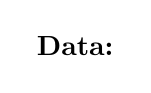
\begin{tikzpicture}[x=1cm,y=0.3cm]
		\node[] (a1) {\textbf{Data:}};			
		\end{tikzpicture}
		}
	\end{minipage}%
	\begin{minipage}{0.35\textwidth}
		\centering
		\subfloat[Dependency among features and prediction]{
			\scalebox{0.4}{	
				\begin{tikzpicture}[x=1.5cm,y=0.3cm]
				% Define nodes
				\node[latent,scale=2] (a1) {$\textrm{age}$} ; %
				\node[obs, scale=2, below=of a1, xshift=-2cm] (h) {$\textrm{fitness}$}; %
				\node[obs, scale=2, below=of a1, xshift=2cm] (i) {$\textrm{income}$}; %
				\node[obs, scale=2, below=of h, xshift=2cm] (p) {$\widehat{Y}$}; %			
				%%add edge
				\edge[] {a1} {h,i} ;
				\edge[] {h,i} {p} ;
				\end{tikzpicture}
			}	
			\label{fairness_fairXplainer_fig:dag_age_income_fitness}}
	\end{minipage}%
	\begin{minipage}{0.4\textwidth}
		\centering
		\subfloat[Age-dependent distributions of non-sensitive features]{\includegraphics[scale=0.4]{figures/fairness/fif/sanity_distribution}
		\label{fairness_fairXplainer_fig:distribution_example}}
	\end{minipage}

	\begin{minipage}[t]{0.13\textwidth}
		\scalebox{1}{	
			
\begin{tikzpicture}[x=1cm,y=0.3cm]
			\node[] (a1) {\textbf{Classifier:}};			
			\end{tikzpicture}
		}
	\end{minipage}%
	\begin{minipage}{0.43\textwidth}
		\centering
		\subfloat[Decision tree (DT$ 1 $)]{
			\scalebox{0.45}{	
				\begin{tikzpicture}[x=1cm,y=1.8cm]
				\node [box, scale=1.5]                                    (p)      {fitness $\geq 0.61$};
				\node [scale=1.5, box, below= of p, xshift=-2.1cm, yshift=1.2cm]    (a1)    {income\\ $\geq 0.29$};
				\node [scale=1.5, box, below= of p, xshift=2.1cm, yshift=1.2cm]     (a2)    {income $\geq 0.69$};
				\node [scale=1.5,below= of a1, xshift=-1.5cm, yshift=0.8cm]  (a11)    { $\widehat{Y}= 1$};
				\node [scale=1.5,below= of a1, xshift=1.5cm, yshift=0.8cm]   (a12)    { $\widehat{Y}=0 $};
				\node [scale=1.5,below= of a2, xshift=-1.5cm, yshift=0.8cm]  (a21)    { $\widehat{Y}= 1$};
				\node [scale=1.5,below= of a2, xshift=1.5cm, yshift=0.8cm]  (a22)    { $\widehat{Y}= 0$};
				%
				\path [line] (p) -|         (a1) node [scale=1.5,midway, above]  {Y};
				\path [line] (p) -|         (a2) node [scale=1.5,midway, above]  {N};
				\path [line] (a1) -|       (a11) node [scale=1.5,midway, above]  {Y};
				\path [line] (a1) -|       (a12) node [scale=1.5,midway, above]  {N};
				\path [line] (a2) -|       (a21) node [scale=1.5,midway, above]  {Y};
				\path [line] (a2) -|       (a22) node [scale=1.5,midway, above]  {N};
				\end{tikzpicture}}
			\label{fairness_fairXplainer_fig:dt_original}}
	\end{minipage}%
	\begin{minipage}{0.45\textwidth}
		\centering
		\subfloat[Decision tree with an affirmative action (DT$ 2 $)]{
			\scalebox{0.45}{	
				\begin{tikzpicture}[x=1cm,y=1.8cm]
				\node [box, scale=1.5]                                    (p)      {fitness $\geq 0.61$};
				\node [scale=1.5, box, below= of p, xshift=-2.1cm, yshift=1.2cm]    (a1)    {income\\ $\geq 0.29$};
				\node [scale=1.5, box, below= of p, xshift=2.1cm, yshift=1.2cm, fill=affirmative]     (a2)    {income $\geq 0.55$};
				\node [scale=1.5,below= of a1, xshift=-1.5cm, yshift=0.8cm]  (a11)    { $\widehat{Y}= 1$};
				\node [scale=1.5,below= of a1, xshift=1.5cm, yshift=0.8cm]   (a12)    { $\widehat{Y}=0 $};
				\node [scale=1.5,below= of a2, xshift=-1.5cm, yshift=0.8cm]  (a21)    { $\widehat{Y}= 1$};
				\node [scale=1.5,below= of a2, xshift=1.5cm, yshift=0.8cm]  (a22)    { $\widehat{Y}= 0$};
				%
				\path [line] (p) -|         (a1) node [scale=1.5,midway, above]  {Y};
				\path [line] (p) -|         (a2) node [scale=1.5,midway, above]  {N};
				\path [line] (a1) -|       (a11) node [scale=1.5,midway, above]  {Y};
				\path [line] (a1) -|       (a12) node [scale=1.5,midway, above]  {N};
				\path [line] (a2) -|       (a21) node [scale=1.5,midway, above]  {Y};
				\path [line] (a2) -|       (a22) node [scale=1.5,midway, above]  {N};
				\end{tikzpicture}}	
			
			\label{fairness_fairXplainer_fig:dt_affirmative}}
	\end{minipage}

	\begin{minipage}[t]{0.07\textwidth}
		%\vspace{-2em}
		\scalebox{1}{	
			
\begin{tikzpicture}[x=1cm,y=0.3cm]
			\node[] (a1) {\textbf{FIF:}};			
			\end{tikzpicture}
		}
	\end{minipage}%
	\begin{minipage}{0.46\textwidth}
		\centering
		\subfloat[Fairness influence functions (FIF) for DT$ 1 $]{\includegraphics[scale=0.42]{figures/fairness/fif/fif_example}
		\label{fairness_fairXplainer_fig:fif_original}}	
	\end{minipage}%
	\begin{minipage}{0.5\textwidth}
		\centering
		\subfloat[Modified FIFs for DT$ 2 $]{\includegraphics[scale=0.42]{figures/fairness/fif/fif_example_affirmative_action}
		\label{fairness_fairXplainer_fig:fif_affirmative}}
	\end{minipage}
%\vspace*{-.5em}
	\caption{FIFs of input features to investigate the bias (statistical parity) of a decision tree predicting the eligibility for health insurance using age-dependent features `fitness' and `income'. An affirmative action reduces bias as corresponding FIFs reflect it.}
	\label{fairness_fairXplainer_fig:fair_example_fif}
	%\vspace{-1.2em}
\end{figure}
